\chapter{\textbf{Contexte général du projet}}

\section{Introduction}

Comme en littérature pour comprendre un mot, il faut recourir à son contexte, de même comprendre un projet nécessite la compréhension de son contexte. Une bonne connaissance de ce dernier permet d’avoir une vision globale de la problématique traitée. C’est donc l’objectif de ce chapitre. Pour l’atteindre, nous allons d’abord présenter l’entreprise où nous avons effectué notre stage. Ensuite, nous ferons une présentation générale du sujet. Enfin, nous verrons la méthodologie de travail adoptée.

\section{Présentation de l'entreprise}

Notre projet de fin d’études a été réalisé au sein d’une jeune et dynamique entreprise marocaine dont le siège se trouve dans la ville de Casablanca. Il s’agit de l’organisme \textbf{KF2Y Consulting}. Fondée en 2010, KF2Y met à la disposition de ses clients un ensemble de compétences et d’experts, pour le déploiement, la maîtrise et l’optimisation des systèmes d’information. L’entreprise propose aux autres entreprises de l'ensemble des secteurs économiques une approche nouvelle qui conjugue l'utilisation de méthodes novatrices et de bonnes pratiques, le recours à la technologie et l'expertise de son capital humain. Pour poursuivre son développement, KF2Y a misé sur 2 pôles:
    \begin{itemize}
        \item[•] \textbf{L’activité Consulting}: 
        ce pôle est né du rapprochement de professionnels du conseil en management et systèmes d’information avec une expertise technologique qui consiste à aider ses clients, qu’ils soient entreprises privées, administrations publiques ou organisations non gouvernementales, à créer de la valeur via la construction et l’implémentation de solutions technologiques avec une ambition de construire des relations pérennes avec ses  clients-partenaires afin de mieux les connaître, mieux anticiper leurs besoins et mieux les servir. Cela se manifeste par la création de valeur ajoutée chez ses clients au niveau des ressources internes ou par une activité de sourcing qui consiste à intervenir dès la phase de recrutement de la ressource pour répondre à un besoin de mission chez nos clients.
        \item[•] \textbf{L’activité Recherche et Développement}: elle vise à mobiliser des ressources internes dans une optique de création des solutions innovantes cherchant à répondre à un paramètre clé de cette mutation économique et digitale vu par le monde.
    \end{itemize}
 KF2Y Consulting couvre un champ d’applications très large et varié tel que :
    \begin{enumerate}
        \item[•] \textbf{Développement IT:} l'entreprise développe pour ses partenaires des applications mobiles et web en utilisant les technologies comme \textbf{Java EE, Angular, Angular JS, .Net, C\#, PL/SQL, SQL, ABAP/4, PHP, Python, Flutter};
        \item[•] \textbf{ERP / Intégration de progiciels}
        \item[•] \textbf{Qualité logiciel et Testing}
        \item[•] \textbf{Big Data et Machine Learning}
        \item[•]  \textbf{Conseil et formation}
    \end{enumerate}
Dans chacun de ces domaines d'action, on retrouve des groupes de personnes qui travaillent sur des projets innovants. En ce qui concerne notre projet, nous avons collaboré avec les membres de l'\textbf{équipe Big Data et Machine Learning}.


La branche Big Data et Machine Learning est une nouvelle branche au sein de l’entreprise. Elle a été créée pour répondre aux besoins sans cesse croissants des systèmes intelligents. L’équipe attachée à cette branche est composée d’\textbf{un manager qui suit l’avancée des projets}, d’\textbf{un responsable qui conduit techniquement les projets} et de certains \textbf{développeurs qui réalisent des applications} intégrant des algorithmes de Big Data et de Machine Learning.
\section{Présentation du projet}
Ces dernières années au Maroc, le nombre des véhicules en circulation ne cesse de croître rapidement. Ceci provoque généralement des violations et de l'anarchie dans le trafic routier. La reconnaissance automatique des plaques d’immatriculation devient donc une urgence. Certes il existe déjà sur le marché des outils qui permettent de lire automatiquement les plaques d’immatriculation. Toutefois, ceux-ci (appelés souvent ANPR) ne prennent pas toujours en compte la particularité des plaques marocaines. \textbf{\textit{Quelles sont donc les caractéristiques de ces plaques ?}}

    \subsection{Caractéristiques des plaques marocaines}
    Généralement sous forme de rectangle ou carrée, la plaque d’immatriculation marocaine est un outil permettant d’identifier les véhicules enregistrés au Maroc. Depuis l’an 2000, les immatriculations doivent respecter une nouvelle norme. Cette nouvelle configuration est composée d’une série de cinq chiffres allant de \textbf{1 à 99 999} qui correspond au numéro d’enregistrement de la voiture. Une lettre de l’alphabet arabe est incrémentée au milieu de la plaque de contrôle, ce dernier prend en compte le numéro d’enregistrement de l’automobile. Pour conclure la combinaison alphanumérique de la plaque minéralogique marocaine, le nouveau système d’immatriculation en vigueur actuellement dans le royaume chérifien termine la combinaison par l’identifiant de la préfecture d’émission de la plaque. Ces numéros vont de \textbf{1 à 89}. Donc les plaques sont maintenant du style \textbf{\#\#\#\#\# | A | \#\#}. Elles ont un fond blanc et les lettres sont en noir.Selon le \href{http://www.equipement.gov.ma/Transport-routier/Carte-grise/Pages/Differents-modeles-de-plaques-d-immatriculation-.aspx}{ministère de l'Equipement, du transport, de la logistique et de l'eau} \cite{mineq}, voici les différents \textbf{modèles de plaques d'immatriculation valides} au Maroc:
        \begin{figure}[H]
            \begin{subfigure}{0.3\textwidth}
                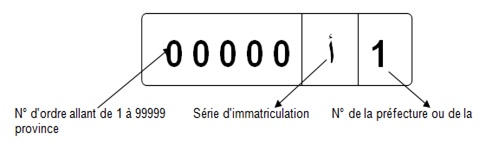
\includegraphics[width=\textwidth]{plaqueVehiculeAutomobile}
                \caption{Modèle sur 1 ligne pour les véhicules automobiles}
            \end{subfigure}
            \hfill
            \begin{subfigure}{0.3\textwidth}
                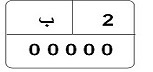
\includegraphics[width=\textwidth]{plaqueVehiculeAutomobileArriere}
                \caption{Modèle sur 2 lignes pour les véhicules automobiles}
            \end{subfigure}
            \hfill
            \begin{subfigure}{0.3\textwidth}
                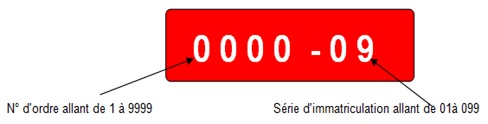
\includegraphics[width=\textwidth]{plaqueRemorqueSup750}
                \caption{Modèle pour les remorques d'un PTAC > 750 Kg}
            \end{subfigure}

            \begin{subfigure}{0.3\textwidth}
                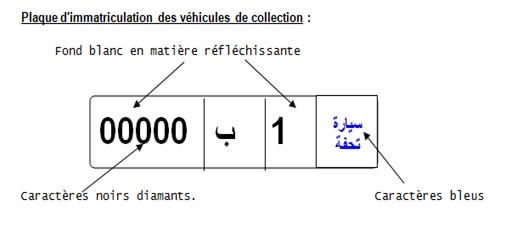
\includegraphics[width=\textwidth]{plaqueVoitureCollection}
                \caption{Modèle pour les véhicules de collection}
            \end{subfigure}
            \hfill
            \begin{subfigure}{0.3\textwidth}
                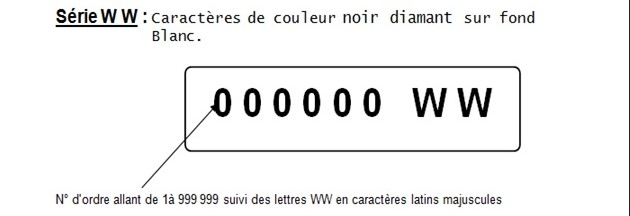
\includegraphics[width=\textwidth]{plaqueSerieWW}
                \caption{Modèle dans la série spéciale WW}
            \end{subfigure}
            \hfill
            \begin{subfigure}{0.3\textwidth}
                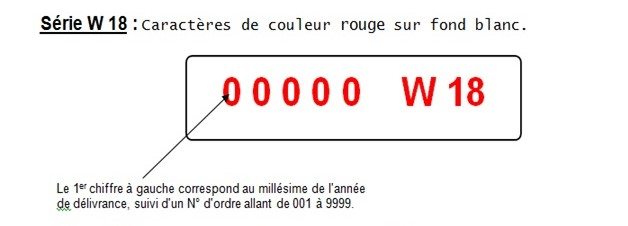
\includegraphics[width=\textwidth]{plaqueSerieW18}
                \caption{Modèle dans la série spéciale W18}
            \end{subfigure}

            \begin{subfigure}{0.3\textwidth}
                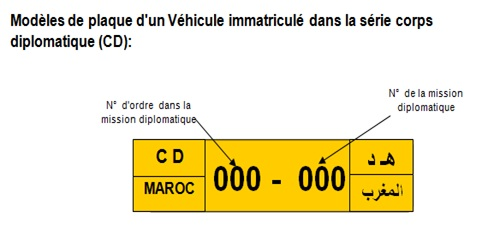
\includegraphics[width=\textwidth]{plaqueVehiculeCorpsDiplomatique}
                \caption{Modèle pour les véhicules de corps diplomatique}
            \end{subfigure}
            \hfill
            \begin{subfigure}{0.3\textwidth}
                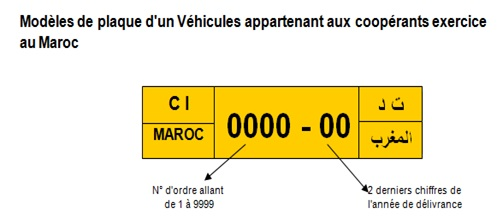
\includegraphics[width=\textwidth]{plaqueVehiculeCooperants}
                \caption{Modèle pour les véhicules des coopérants}
            \end{subfigure}
            \hfill
            \begin{subfigure}{0.3\textwidth}
                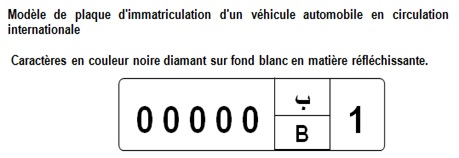
\includegraphics[width=\textwidth]{plaqueVehiculeACirculationInternationale}
                \caption{Modèle pour les véhicules en circulation internationale}
            \end{subfigure}
            \caption{Modèles de plaques d'immatriculation marocaines}
        \end{figure}
    En considérant ces caractéristiques, notre système doit prendre en entrée des images ou vidéos de véhicules au Maroc et être capable d'extraire l'ensemble des  numéros de plaques s'y trouvant pour un enregistrement dans une base de données.

    \subsection{Problèmatique et Objectifs du projet}
    Le projet surlequel nous avons travaillé est la résultante de deux constats majeurs faits sur le trafic routier au Maroc:
    \begin{enumerate}
            \item Le premier est lié à l’\textbf{augmentation rapide du nombre de véhicules en circulation dans le Royaume chérifien}.  Cette croissance accroît l’ampleur des problèmes liés au trafic routier comme le vol des voitures, les congestions, la violation des codes routiers et bien d’autres encore. 
            \item Le second  est lié au \textbf{système actuel de gestion de parking dit intelligent} et particulièrement la méthode actuelle pour ouvrir la barrière afin d'accéder à la zone de stationnement. Pour le moment, la plupart des systèmes implémentés dans le pays utilisent régulièrement des cartes \acrshort{rfid}. Ce qui rend le système pas vraiment automatisé de bout en bout.
        \end{enumerate}
    Face à ces constats, l’entreprise KF2Y Consulting dans sa démarche de création des villes intelligentes destinées au marché marocain a voulu mettre en place un système automatique de bout en bout pour la reconnaissance des plaques d’immatriculation marocaines.  Cette mission nous a donc été confiée dans le cadre de notre projet de fin d'études avec les objectifs suivant:
        \begin{enumerate}
            \item \textbf{Mettre en place un système \acrshort{anpr} spécifique aux plaques marocaines appelé \textit{MoPlaZer} performant (rapide et précis)}: Ce système doit être en mesure de localiser d’une part  les plaques d’immatriculation sur une image ou une vidéo et d’autre part extraire sous format alphanumérique leur numéro d’immatriculation.
            \item \textbf{Concevoir et développer une application mobile qui intègre le système}: L’application doit proposer deux modes de traitement
                \begin{itemize}
                    \item \textbf{Un mode statique}: Ici le système \acrshort{moplazer} traite les images fixes prises par une capture ou récupérées dans l’appareil mobile.
                    \item \textbf{Un mode temps réel}: Ici le système traite les séquences d’images continues (mode vidéo) à travers la caméra de l’appareil mobile
                \end{itemize}
            \item \textbf{Intégrer le système \acrshort{moplazer} dans un système embarqué pour un smart parking}: En effet le système \acrshort{moplazer} devra fournir sous format texte le numéro des plaques d’immatriculation des véhicules qui viennent à l’entrée du parking. Par la suite une vérification de l’existence du matricule détecté dans une base de données est faite. Dans le cas où le matricule se trouve dans la base de données, on déclenche l’ouverture de la barrière qui donne accès aux zones de stationnement.
        \end{enumerate}



\section{Conduite de projet}
Pour réussir tout projet, il est indispensable de mettre en place une bonne méthodologie de travail. Une bonne méthodologie de travail est celle qui donne à une équipe de pouvoir livrer un produit tout en respectant les délais, les budgets et les ressources disponibles. Par ailleurs, il faut associer à toute bonne méthodologie des outils d'organisation et de communication qui l'implémentent concrètement.
    \subsection{Méthodologie de travail}
    Dans le domaine de l’informatique, on retrouve plusieurs méthodologies de gestion des projets qui peuvent être classées principalement dans deux grands groupes:
        \begin{itemize}
            \item[•] \textbf{Les méthodes traditionnelles: }encore désignées comme classiques ou waterfall (cascade), ces méthodologies suivent la logique d’une chute d’eau. En appliquant cette méthode, l’équipe de projet suit un cahier de charges à la lettre et travaille sur la totalité du projet jusqu’à sa livraison. Rigide, elle ne prévoit pas des interactions permanentes avec le client qui ne pourra recevoir son produit qu’à la fin du projet. Toutefois, elle possède l’avantage d’être simple à mettre en œuvre.
            \item[•] \textbf{Les méthodes agiles: }plus efficaces et moins rigides que les méthodes classiques, les méthodes agiles placent les besoins du client au centre des priorités du projet. Elles offrent une plus grande flexibilité et une meilleure visibilité dans la gestion du projet, ce qui permet à l'équipe d'être plus réactive aux attentes du client. Le projet est ainsi découpé en mini-projets, chacun nécessitant la validation du client pour passer au suivant. Le dialogue avec le client est privilégié, les retours et les ajustements sont possibles. On prend davantage en considération l'évolution des besoins du client. Parmi les méthodes Agile largement connues, nous pouvons citer l'\textbf{\acrfull{xp}},
            \textbf{Scrum}, \textbf{\acrfull{fdd}}, \textbf{Lean Software Development}, \textbf{\acrfull{aup}}, \textbf{\acrfull{dsdm}}.
        \end{itemize}

        Toutes les méthodologies sus-citées possèdent chacune des avantages et des inconvénients. Ainsi quand il s’agit de choisir une méthode, nous ne cherchons pas la meilleure mais la plus adaptée à notre projet. Et pour ce qui concerne notre projet, puisque d’une part un cahier de charges fixe n’est pas déterminé dès le départ et d’autre part les besoins du client sont susceptibles de changer suivant l’avancement du projet, nous avons opté pour la souplesse de la méthodologie Agile et plus particulièrement la méthode Scrum.
        
        Co-fondé dans \textbf{les années 1990} par \textbf{Ken Schwaber} et \textbf{Jeff Sutherland}, Scrum est un cadre dans lequel les gens peuvent résoudre des problèmes adaptatifs complexes, tout en fournissant de manière productive et créative des produits de la plus haute valeur possible. En bref, Scrum a besoin d'un Scrum Master pour favoriser un environnement où : 
            \begin{enumerate}
                \item Un Product Owner ordonne le travail à faire pour résoudre un problème complexe dans le Product Backlog. 
                \item La Scrum Team transforme une sélection de ce travail en un Increment de valeur lors d'un Sprint. 
                \item La Scrum Team et ses parties prenantes inspectent les résultats et s'adaptent pour le prochain Sprint. 
                \item Répéter
            \end{enumerate}
            \begin{figure}[H]
                \centering
                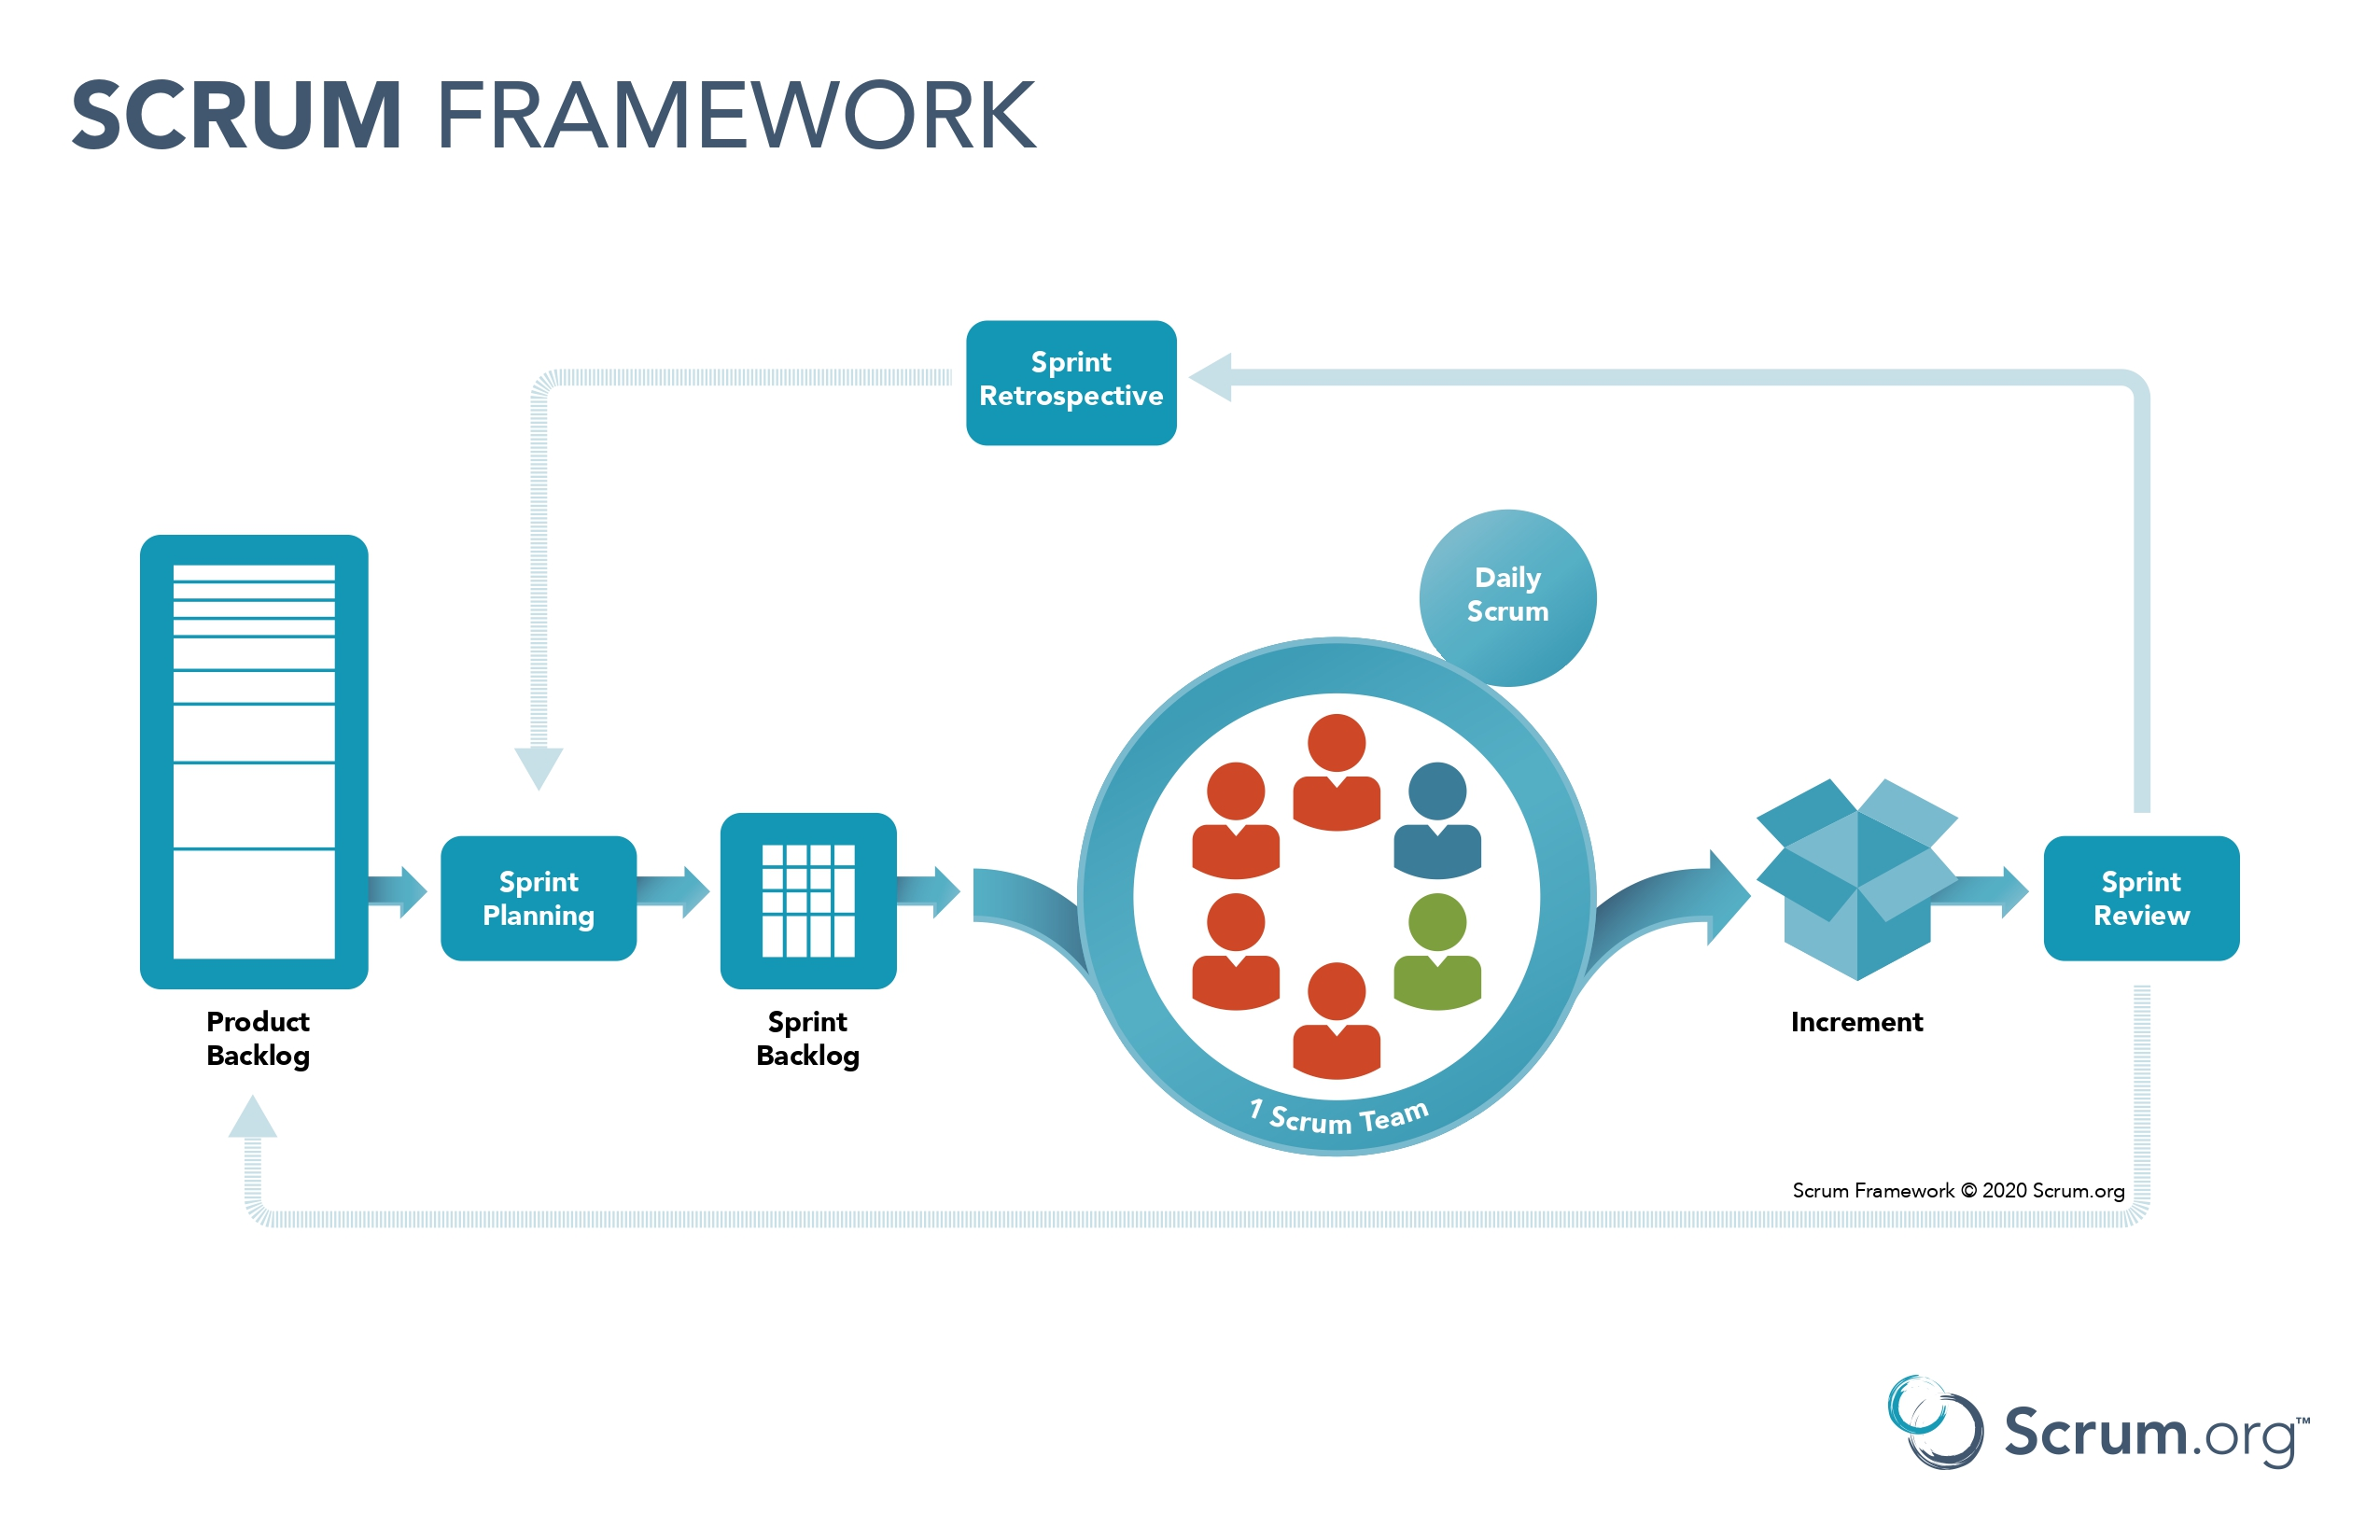
\includegraphics[scale=0.3]{scrum}
                \caption{Le cadre de travail SCRUM}
            \end{figure}
        Pour une implémentation réelle, le framework Scrum nécessite le regroupement et le respect d’un certain nombre d'éléments qui font sa particularité. Ce sont notamment:

        \begin{itemize}
            \item Les \textbf{piliers: } Scrum dispose de 3 grands piliers empiriques à savoir: la \textbf{transparence}, l' \textbf{inspection},  l'\textbf{adaptation}.
            \item Les \textbf{valeurs: }pour réussir bien un projet Scrum, les membres de l'équipe doivent être capables de respecter cinq valeurs fondamentales: l' \textbf{engagement} à suivre les objectifs fixés, le \textbf{focus} sur le but commun, l' \textbf{ouverture} face aux difficultés professionnelles, le \textbf{respect mutuel} entre les collaborateurs et enfin le \textbf{courage} pour une exécution de manière excellente des tâches et la relève des challenges.
            \item Les \textbf{événements: } 4 (quatres) événements majeurs permettant la création de la régularité font la méthodologie Scrum: les \textbf{Sprints} d'une durée fixe allant de 2 semaines à 1 mois au plus, le \textbf{Sprint Planning} qui lance un sprint, le \textbf{Daily Scrum} pour inspecter les progressions, le \textbf{Sprint Review} pour analyser les résultats et déterminer les adaptations futures.
            \item Les \textbf{artefacts: }ceux-ci représentent un travail ou une valeur. Nous avons trois artefacts Scrum: le \textbf{\textit{Product Backlog}} qui exprime l'objectif du produit, le \textbf{\textit{Sprint Backlog}} définit l'objectif du sprint et l' \textbf{\textit{Increment}} qui établit la signification d'un \textit{"sprint terminé ou fini"}.
            
            \item L' \textbf{équipe: }Scrum s'organise toujours autour d'une petite équipe d'au plus 10 (dix) personnes. Cette équipe est composée des \textbf{\textit{Developers}} qui implémentent concrétement chaque incrément d'un sprint, le \textbf{\textit{Product Owner}} qui détaille les objectifs du produit à livrer, le \textbf{\textit{Scrum Master}} qui met en place le Scrum et assure l'efficacité de l'équipe.
        \end{itemize}
    Pour ce qui concerne notre projet, notre Scrum Team était constituée comme suit:
        \begin{table}[H]
            \centering
            \begin{tabular}{|l|l|}
                \hline
                \rowcolor{Gray}
                \textbf{Fonction} & \textbf{Noms et Prénoms} \\ \hline
                \textbf{Product Owner} & \textbf{M. Youssef} \\ \hline
                \textbf{Scrum Master} & \textbf{M. Marouane GHOULAMI} \\ \hline
                \textbf{Developers} & \textbf{M. Hisdaele KAMGA} \\ \hline  
            \end{tabular}
            \caption{Scrum Team du projet}
        \end{table}
    Nous avons suivi des sprints d'une semaine. La définition des objectifs sont définies en début de semaine. À la fin de la semaine, un rapport sur le sprint achevé est effectué et contient l'état d'avancement du projet ainsi que les perspectives pour le prochain sprint.

    \subsection{Outils d'organisation et de communication}
        Toute équipe de projet doit savoir d’une part s’organiser et d’autre part communiquer. Avec l’essor de l’informatique, ces tâches essentielles deviennent plus faciles. En effet, il existe plusieurs plateformes gratuites qui permettent aussi bien de planifier et suivre les activités d’un projet que de faciliter la communication au sein de groupe de travail. Pour notre projet, nous avons opté pour des outils simples et largement connus:

        \begin{enumerate}
            \item \textbf{Trello: }lancé en \textbf{septembre 2011}, Trello est un outil en ligne de gestion de projet inspiré de la méthode Kanban de Toyota. Il repose sur une organisation des projets en planches listant des cartes, chacune représentant des tâches. Les cartes sont assignables à des utilisateurs et sont mobiles d'une planche à l'autre, traduisant leur avancement. Ainsi Trello va nous servir à représenter les différentes informations sur les sprints en cours, effectués.
            \item \textbf{TeamGantt: } pour pouvoir planifier les différentes tâches et les visualiser, nous avons utilisé le \textbf{diagramme de Gantt}. C'est un outil pour l'ordonnancement et la gestion de projet. Elle permet d'un coup d'oeil de \textbf{déterminer les dates de début et de fin des tâches}, d'\textbf{identifier les marges existantes sur certaines tâches} et de \textbf{connaître l'état d'avancement du projet en général}. Pour créer ce diagramme de Gantt pour notre projet, nous avons travaillé avec la plateforme en ligne TeamGantt. Elle permet facilement de placer de nouvelles tâches avec leurs dates de début et de fin sur un diagramme de Gantt.
            \item \textbf{Skype: }c'est un logiciel qui permet de faire des échanges téléphoniques, vidéo et des messages via internet. Nous l'avons utilisé au cours de notre projet pour échanger des messages et partager certains fichiers ou liens utiles pour l'avancement des travaux.
            \item \textbf{Microsoft OutLook: }c'est un gestionnaire d'informations personnelles et un client de courrier électronique propriétaire édité par Microsoft. Ce logiciel informatique fait partie de la suite bureautique Microsoft Office. Bien qu'il soit principalement utilisé en tant qu'application de courrier électronique, il propose aussi un calendrier et un gestionnaire de tâche et de contact. Nous avons utilisé ce logiciel pour communiquer officiellement avec le Product Owner et le Scrum Master. A travers cet outil, nous envoyons avec une certaine régularité les rapports d'avancement du projet avec les prochaines perspectives.
            \item \textbf{Microsoft OneNote: }pour les prises de notes importantes, nous avons opté pour Microsoft OneNote. C'est un programme développé par le géant Microsoft qui nous a permis de tracer les avancées journalières.
            \item \textbf{Google Meet: } c'est un outil de vidéoconférence développé par Google. Nous l'avons utilisé pour faire certaines rencontres de mise au point en ligne avec le Manager M. Youssef. 
        \end{enumerate}

        \begin{figure}[H]
            \begin{subfigure}{0.3\textwidth}
                \centering
                
\includegraphics[width=\textwidth]{trello.png}
                \caption{Trello}
            \end{subfigure}
            \hfill
            \begin{subfigure}{0.3\textwidth}
                \centering
                
\includegraphics[width=\textwidth]{teamgantt.jpg}
                \caption{TeamGantt}
            \end{subfigure}
            \hfill
            \begin{subfigure}{0.3\textwidth}
                \centering
                
\includegraphics[width=0.3\textwidth]{GoogleMeet}
                \caption{Google Meet}
            \end{subfigure}

            \begin{subfigure}{0.3\textwidth}
                \centering
                
\includegraphics[width=0.3\textwidth]{microsoftOutlook.png}
                \caption{Microsoft OutLook}
            \end{subfigure}
            \hfill
            \begin{subfigure}{0.3\textwidth}
                \centering
                
\includegraphics[width=0.3\textwidth]{oneNote.png}
                \caption{Microsoft OneNote}
            \end{subfigure}
            \hfill
            \begin{subfigure}{0.3\textwidth}
                \centering
                
\includegraphics[width=0.3\textwidth]{skype.png}
                \caption{Skype}
            \end{subfigure}
            

            \caption{Logos des outils d'organisation et de planification}
        \end{figure}


        







\section{Conclusion}
Nous arrivons au terme de ce tout premier et important chapitre. Il nous a permis de mettre en lumière le contexte général dans lequel se situe notre projet de fin d’études. Il en ressort que ce projet s’inscrit dans une démarche innovante de la jeune et dynamique entreprise marocaine KF2Y Consulting. C’est une démarche pour rendre le trafic routier au Maroc plus facile, plus contrôlé et en quelque sorte intelligent. Et ceci à travers la mise en place d’un système rapide et précis de reconnaissance automatique de plaques minéralogiques marocaines qu'on appelle plus techniquement les systèmes \acrshort{anpr}. Si les systèmes ANPR ne sont pas encore très répandus au Maroc, dans le reste du monde ils sont déjà été et continuent à être l'objet de plusieurs études scientifiques depuis plus d’une vingtaine d’années. Nous allons donc consacrer le prochain chapitre à ces études.